\section{Experiments}
\label{sec:experiments}

\begin{table*}[!h]
\caption{Experimental results for two cities: Travel time estimates from road speed profiling and corrective \ac{ML} algorithm for City 1 and City 2 compared using MAPE, RMSE and BIAS.}
\centering
\begin{tabular}{|c|c|c|c|c|c|c|c|}
\hline
\multirow{3}{*}{\textbf{City}} & \multirow{3}{*}{\textbf{Phase}} & \multicolumn{6}{c|}{\textbf{Metric}}                                                                                                                                                                                                                                                                                                                                                                                                                                                          \\ \cline{3-8} 
                               &                                 & \multicolumn{2}{c|}{\textbf{MAPE}}                                                                                                                            & \multicolumn{2}{c|}{\textbf{RMSE}}                                                                                                                            & \multicolumn{2}{c|}{\textbf{Bias}}                                                                                                                            \\ \cline{3-8} 
                               &                                 & \textbf{\begin{tabular}[c]{@{}c@{}}Speed profiles\\ only\end{tabular}} & \textbf{\begin{tabular}[c]{@{}c@{}}After \\ corrective ML \\ algorithm\end{tabular}} & \textbf{\begin{tabular}[c]{@{}c@{}}Speed profiles\\ only\end{tabular}} & \textbf{\begin{tabular}[c]{@{}c@{}}After \\ corrective ML \\ algorithm\end{tabular}} & \textbf{\begin{tabular}[c]{@{}c@{}}Speed profiles \\ only\end{tabular}} & \textbf{\begin{tabular}[c]{@{}c@{}}After \\ corrective ML\\ algorithm\end{tabular}} \\ \hline
\multirow{2}{*}{City $1$}            & Pick up                         & 0.52                                                                   & 0.42                                                                                 & 122.84                                                                 & 100.66                                                                               & 29.97                                                                   & 22.11                                                                               \\ \cline{2-8} 
                               & Drop off                        & 0.21                                                                   & 0.145                                                                                & 261.19                                                                 & 172.61                                                                               & 175.13                                                                  & -6.745                                                                              \\ \hline
\multirow{2}{*}{City $2$}           & Pick up                         & 0.55                                                                   & 0.47                                                                                 & 193.27                                                                 & 162.84                                                                               & 40.05                                                                   & 33.03                                                                               \\ \cline{2-8} 
                               & Drop off                        & 0.27                                                                   & 0.18                                                                                 & 536.17                                                                 & 344.88                                                                               & 349.02                                                                  & 52.11                                                                               \\ \hline
\end{tabular}
\label{table:results}
\end{table*}



In this section, we evaluate the efficacy of road speed profiling, and assess the impact of the corrective Gradient Boosted decision tree~\cite{} algorithm on TTE. We evaluate this for both the phases of a trip commonly known in ride-hailing namely, i) the pickup phase, which is the time taken for the to reach the passenger for pickup after accepting the ride, and ii) drop off phase, which is the duration between passenger pickup and drop-off. Since these two phases have very different distributions, we train two separate ML models for correcting \ac{RSP} based travel time estimates. 

\textbf{Dataset:}
For generating the \ac{RSP} we used driver trajectories from close to $9.5$ million rides in (each)  City~$1$ and City~$2$ spanning 4 weeks. To train the corrective GBDT model for the pick up phase, we used $800$k train and $200$k test samples while  $1.3$ million train and $400$k test samples were used to train the model for the drop off phase.

\textbf{Features:}
The features to train the GBDT models are expected, median, upper and lower bound travel times and the routing distance (for an \ac{OD} pair) along with the minute of the day and day of the week of the trip. The label for the \ac{ML} model is the actual travel time from the origin to destination.

 

The metrics we use to evaluate the performance of the travel time estimates from \ac{RSP} and GBDT models against the actual travel times are as follows: 
\begin{enumerate}
\item \ac{MAPE} given by $\frac{1}{N}\sum_{i=1}^{N} \frac{abs(y_i-y_p)}{y_i}$

\item \ac{RMSE} given by $\sqrt{\frac{1}{N}\sum_{i=1}^{N} (y_i-y_p)^2}$

\item Bias given by $\frac{1}{N}\sum_{i=1}^{N} (y_i-y_p)$
\end{enumerate}
Where $y_i$ and $y_p$ represent the actual and predicted travel times for an \ac{OD} pair.

\subsection{Evaluation}
\label{subsec:results}
In this section we evaluate the performance of \ac{TTE} using the values from just road speed profiling and then followed by the corrective \ac{ML} model.

In Table~\ref{table:results} we summarize the results of road speed profiling and the corrective \ac{ML} models for City~$1$ and City~$2$ for the two phases of a cab ride. 

The results clearly show that the performance of both road speed profiling and corrective \ac{ML} model is superior in terms of \ac{MAPE} for the drop off phase compared to the pickup phase this is attributed to the greater uncertainty in the expected route a driver will take to pickup a passenger. We can also ascertain that the corrective \ac{ML} algorithm has significantly improved all the metrics compared to the output from \ac{RSP}. Finally the results of \ac{TTE} for City~$1$ is better than City~$2$ for all metrics considered. This can be attributed to City~$1$ having better infrastructure and lesser vehicle density resulting is less congestion.


\begin{figure}[!tb]
	\centering
	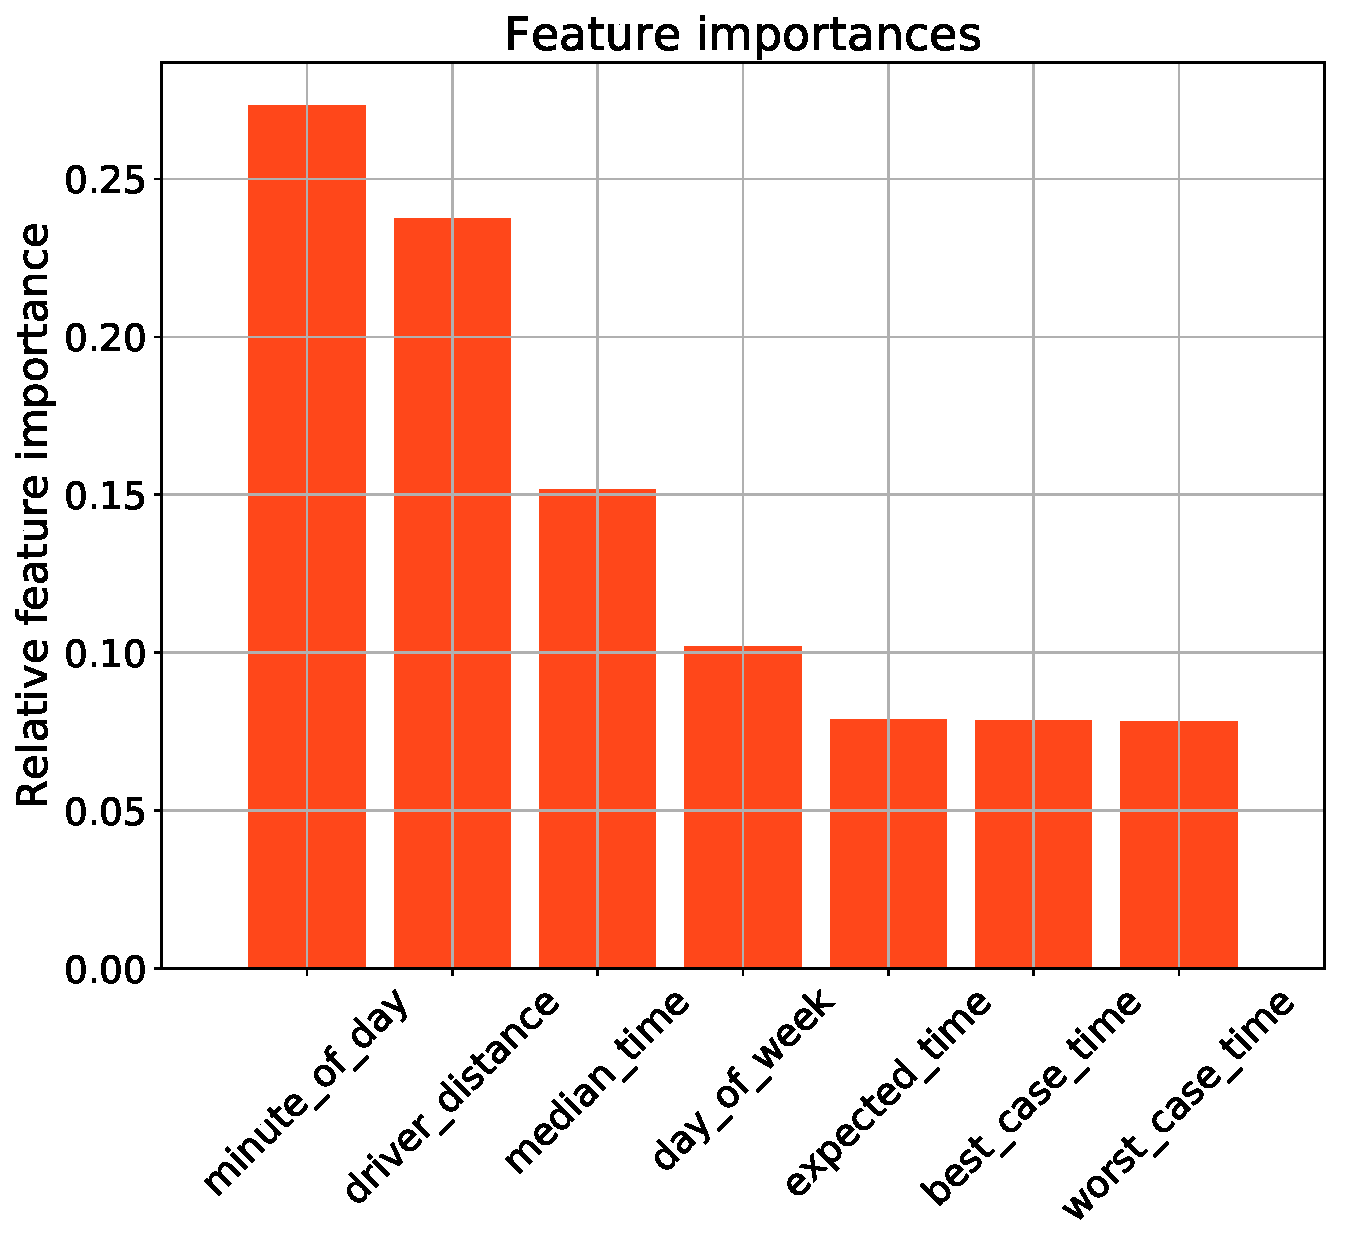
\includegraphics[width=\columnwidth,left,height=6.5cm,keepaspectratio]{images/feauture_importance.pdf}
	
	\caption{Relative feature importance from the GBDT model.}
	\label{fig:xgb-feature-importance}
\end{figure}



Figure~\ref{fig:xgb-feature-importance} shows the feature importance for one of the corrective GBDT models. Note that the order of feature importance in every GBDT model is the same. We see that the features \textbf{minute of the day} and the \textbf{driver distance} are the most important for correcting the \ac{RSP} travel time estimates. The former is important since the \ac{CoV} in speed profiles is dependent upon peak and non peak hours of the day. The driver distance is also an important feature for the corrective \ac{ML} model since we have seen that greater the distance between the \ac{OD} pairs more certain we are about the path that driver will take, thus resulting in better \ac{RSP} travel time estimates. Finally, we also observed that \textbf{median time} obtained from RSPs is also considered among the top-3 important features, proving the contribution of our inferred RSPs.  


\begin{figure}[!tb]
	\centering
	\subfloat[\ac{MAPE} over time of the day]{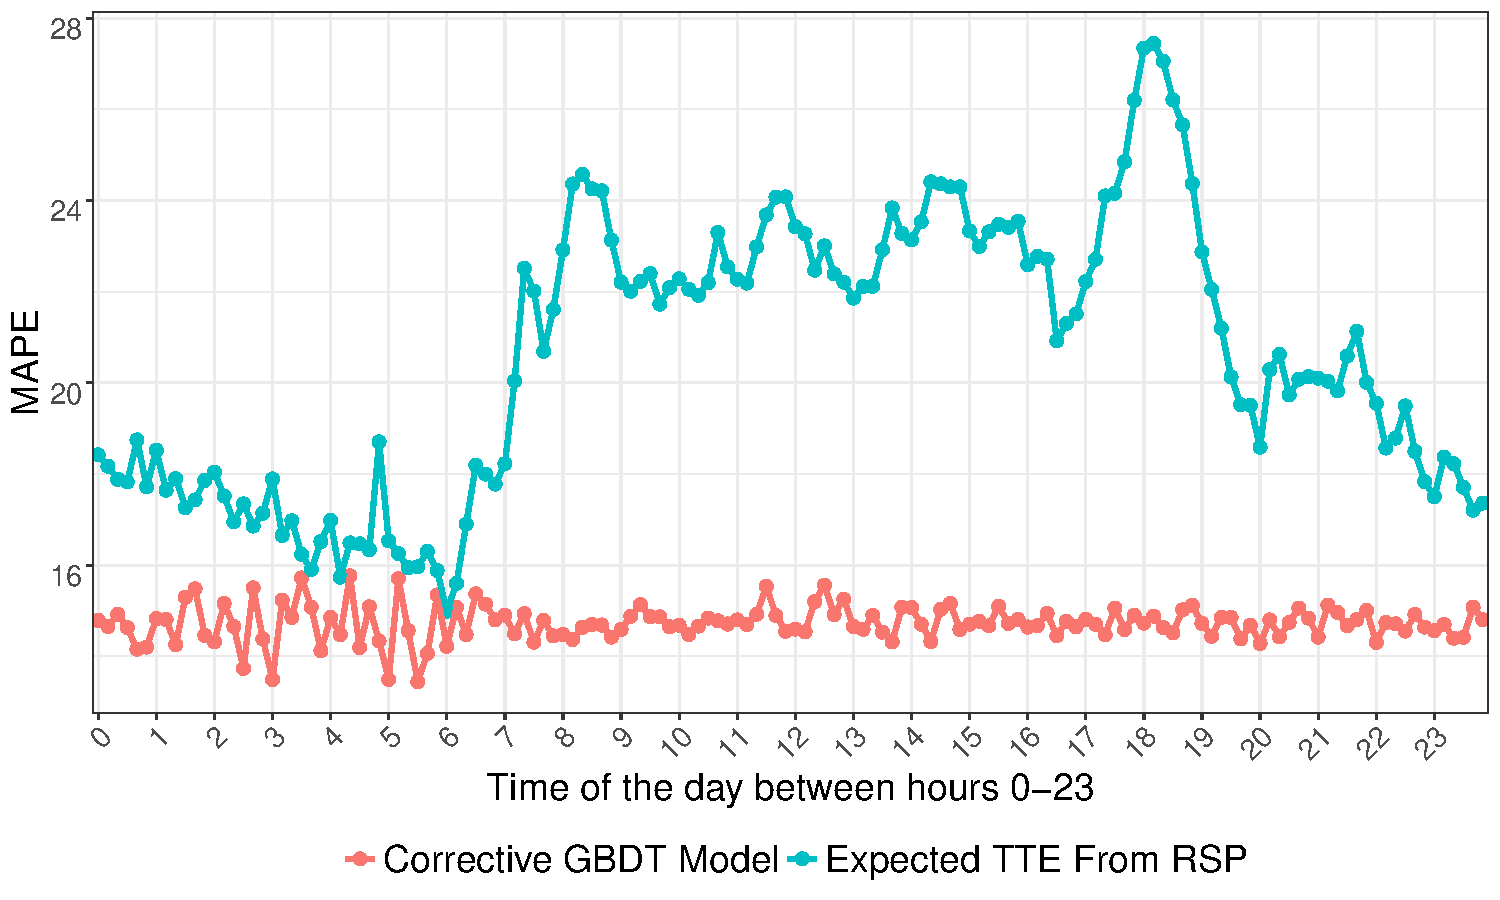
\includegraphics[width=\columnwidth,height=5.6cm,keepaspectratio]{images/ETT-TOD-SG.pdf}\label{fig:compare-rsp-xgboost-tod}}%
	\vfill%
	\subfloat[\ac{MAPE} over buckets (in km).]{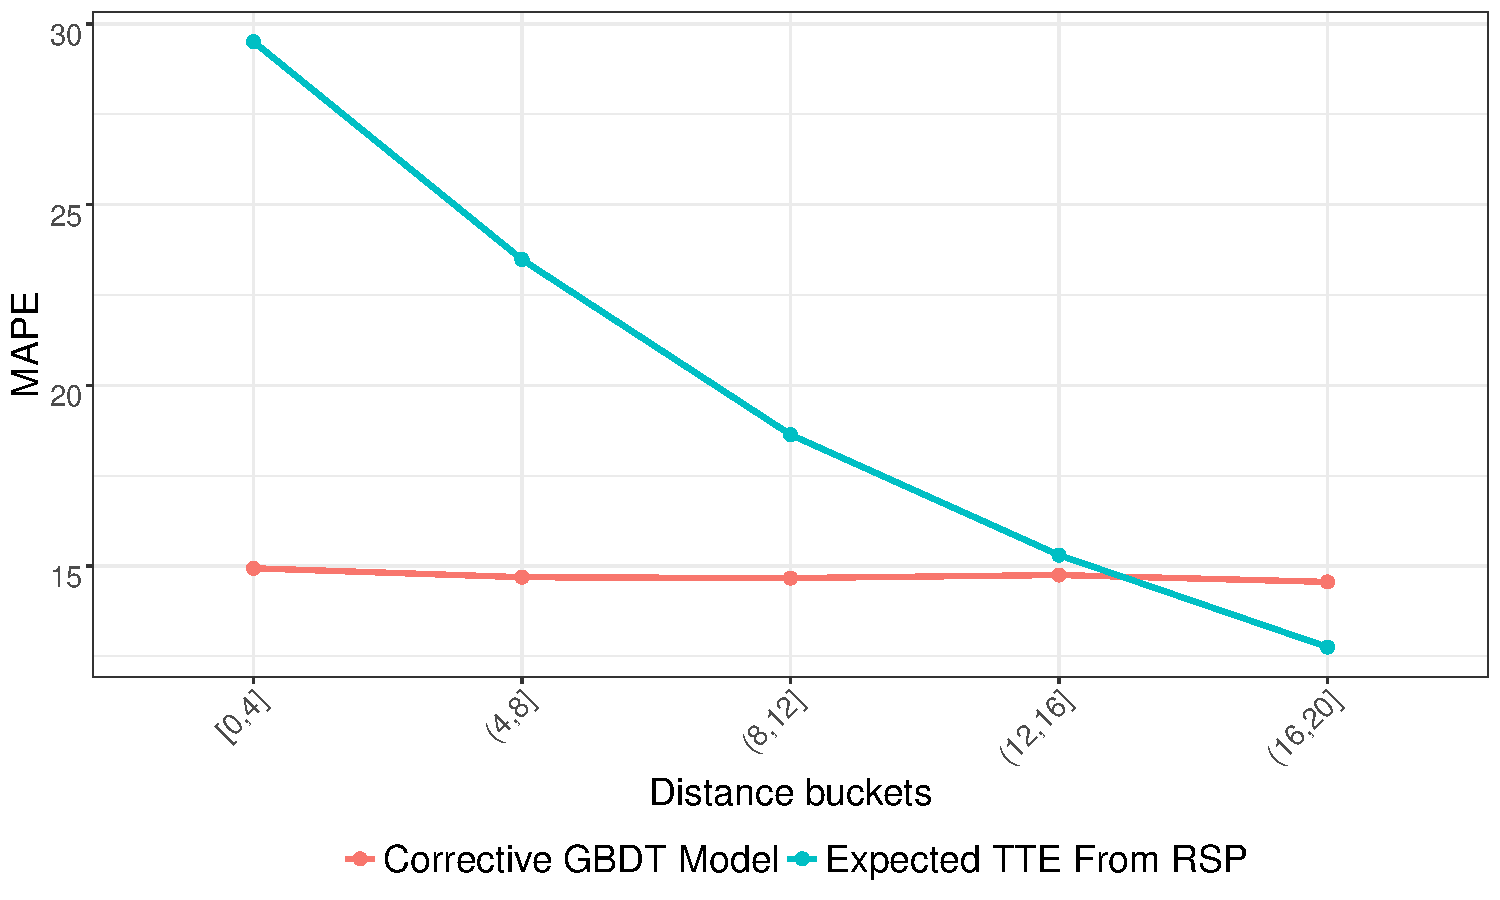
\includegraphics[width=\columnwidth,height=5.6cm,keepaspectratio]{images/ETT-Distance-SG.pdf}\label{fig:compare-rsp-xgboost-distance}}%
	\label{fig:eval-dropoff-sg}
	\caption{\ac{RSP} vs corrective GBDT model for the drop off phase in City $1$}
\end{figure} 

Figure~\ref{fig:compare-rsp-xgboost-tod} compares the performance of the expected travel time from \ac{RSP}  with that of the corrective GBDT model which takes the output of \ac{RSP} as input for City $1$ over an entire day. We can see that travel time estimates from \ac{RSP} have varying accuracy based on time of day. MAPE for estimates during non peak hours is less compared to that of peak hours, which could be attributed to large variance in traffic flow (as discussed in Section~\ref{subsec:speed-disribution}) that is not captured by RSPs, perhaps with the given data. The performance of  GBDT model tends to have less variance over time, indicating that GBDT captures non-linearities in traffic flow and time dependencies well in order to correct the errors in \ac{RSP}. 


Figure~\ref{fig:compare-rsp-xgboost-distance} compares the performance of \ac{RSP} with GBDT model for different distance buckets during the drop off phase for City $1$. We can see that the performance of the expected speed from \ac{RSP} becomes better as the distance of the ride increases. This can be attributed to the fact that we tend to predict the path for an \ac{OD} pairs that are far apart with better accuracy than for OD pairs that are close by. Note that knowing the exact path taken by the driver plays a crucial role in using RSP for TTE. For shorter rides there are multiple paths that can be taken from the origin to destination. This is amplified further by inaccuracies in \ac{OSM}'s routing especially seen for shorter rides. Performance of the GBDT model is again distance invariant. We notice that the performance of the GBDT gets worse than the RSP based estimates for  $16-20$ km distance bucket since we have very few rides in that bucket in our training data. 
This indeed highlights the limitations and merits of GBDT based approach and RSP based approach respectively.  

\begin{figure}[!tb]
	\centering
	\subfloat[\ac{MAPE} over time of the day]{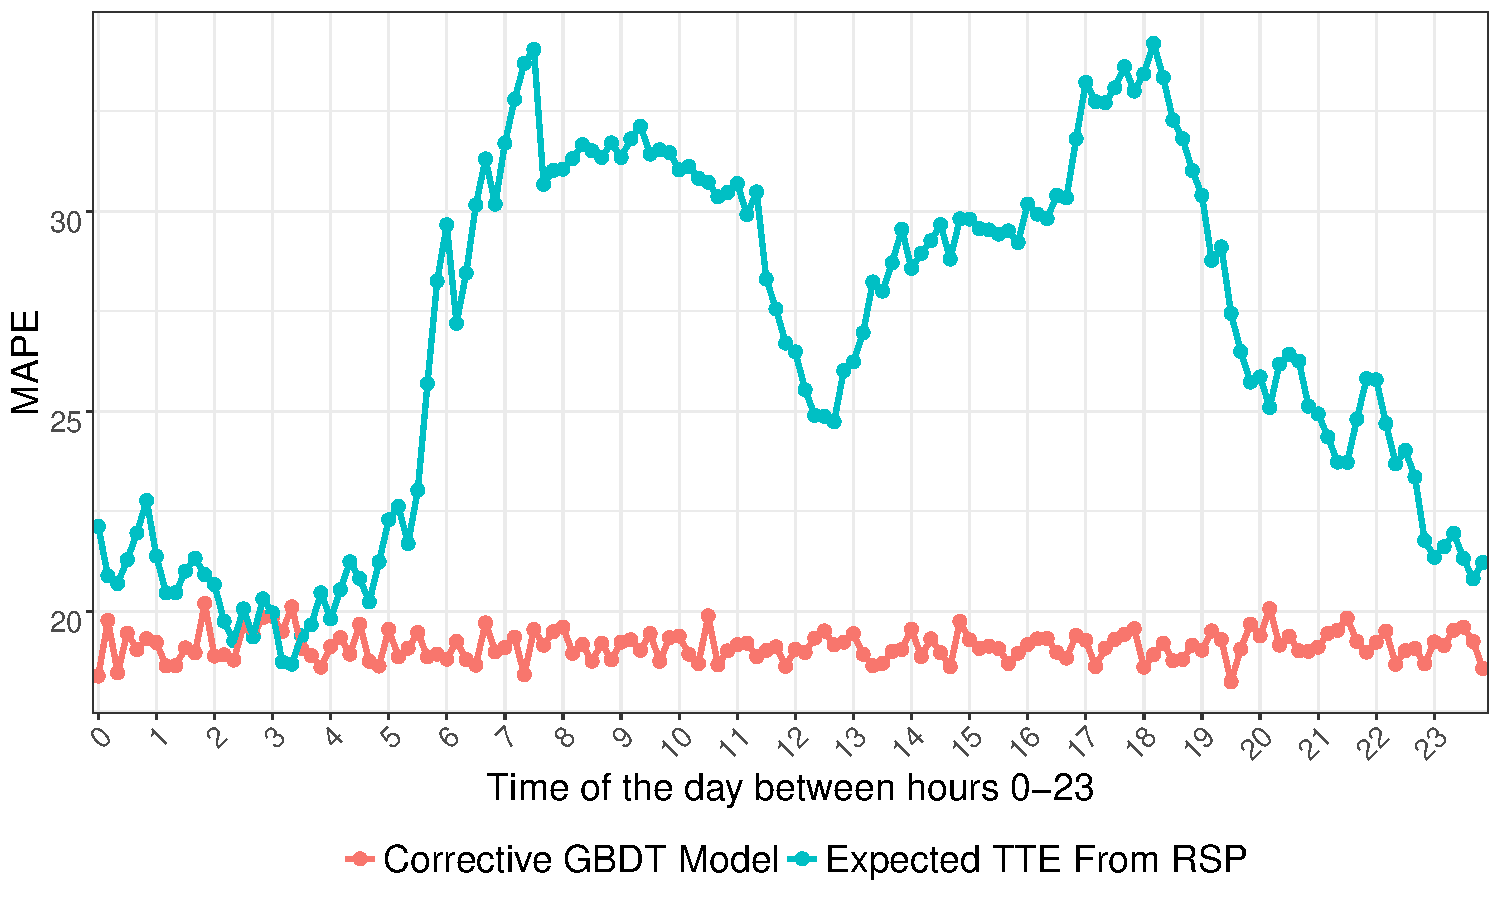
\includegraphics[width=\columnwidth,height=5.6cm,keepaspectratio]{images/ETT-TOD-MNL.pdf}\label{fig:compare-rsp-xgboost-tod-mnl}}%
	\vfill%
	\subfloat[\ac{MAPE} over buckets (in km).]{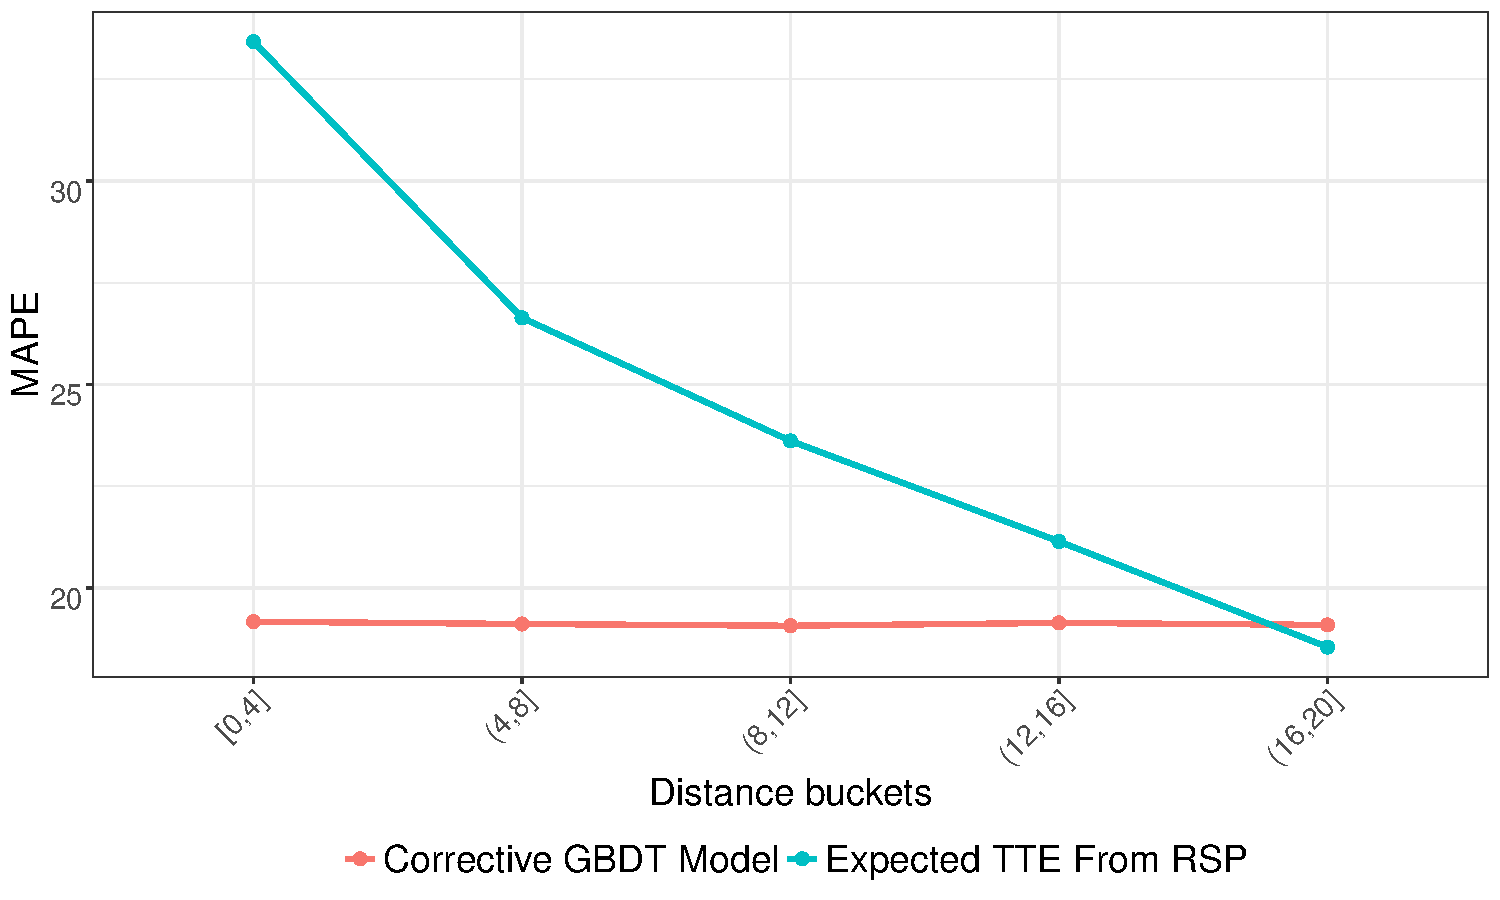
\includegraphics[width=\columnwidth,height=5.6cm,keepaspectratio]{images/ETT-Distance-MNL.pdf}\label{fig:compare-rsp-xgboost-distance-mnl}}%
	\label{fig:eval-dropoff-mnl}
	\caption{\ac{RSP} vs corrective GBDT model for the drop off phase in City $2$}
\end{figure} 

A similar comparison, i.e., performance of the expected travel time from \ac{RSP} vs GBDT based corrective model for the drop off phase in City $2$, 
is presented in figures~\ref{fig:compare-rsp-xgboost-tod-mnl} and~\ref{fig:compare-rsp-xgboost-distance-mnl}. The conclusions that we can derive from the plots for City $2$ are the same for City $1$. As noted in Table~\ref{table:results} we can see that \ac{RSP} estimates and GBDT model performance are inferior for City $2$ compared to City $1$.
